% From Skoltech's requirements:
%
% > The main part includes:
% > - A description of the history and background literature on the subject
% > - Statement of research problem
% > - Statement of methodology
% >     - Design, data collection, analysis, interpretation
% > - Results
% > - Discussion of innovation and research findings
% > 
% > Justification of reseach relevance is mandatory.


\chapter{Overview of the work}

\section{Subject's history and background} \label{sec:history}

In 2017-2018~\cite{nickelKiela17} it came to attention of deep learning community, that for a
Euclidean space of fixed dimension, \( \mathbb{R}^n \) with usual distance
function, there are graphs which cannot be isometrically embedded in it, and
that any graph could be isometrically embedded in a Hyperbolic space.
Sarkar~\cite{sarkar} gives a combinatorial algorithm for approximately
isometric embedding of a tree. This has inspired a number of works using
hyperbolic representations for graph-like data, for instance in language models

\subsection*{Curvature in metric graphs}

Consider a graph that consists of vertices connected by edges. Such a graph is
a metric space -- its points are the nodes of the graph, and distances are
measured in smallest number of edges on has to travel to get from one node to
another.  Now, such distances can behave very wildly, compared to Euclidean
space. For instance, you could have any number of points that are
simulataneosuly nearest neighbours of each other (consider the fully-connected
graph \( K_n \)), whereas in a two-dimensional Euclidean
plane~\cite{howManyNeighbours} the best you can do is three points allocated in
an equilateral triangle. This has immediate implications if you were to define
the notion of ``similarity'' of objects (images or words) in terms of distance
between their embeddings.  For instance, we could say that objects are
``similar'' if the ``distance'' between them is no more than \( 1 \) (an
arbitrarily chosen threshold).  That's a binary relation, and with
graph-distances such relation could well be non-transitive. This is easily seen
in a tree of constant branching factor: the sibling nodes are both ``similar''
to their common immediate parent, but not to each other. For a ``branchy''
enough tree, such relationships simply cannot be modeled by distances between
Euclidean embeddings (of pre-defined dimension).

The reason such isometric embeddings into Euclidean space are impossible for
certain graphs is that these graphs have \emph{curvature} different from that
of Euclidean space. We shall clarify this statement in later sections.

\subsection*{Hyperbolic Neural Networks}

\citet{ganeaHNNs} introduce hyperbolic neural layers which operate on
hyperbolic embeddings and can be arbitrarily stacked into deep networks.  To
save space, we cover this subject in more detail (including references) in the
appendix:~\nameref{appendix:hyperbolics}. \nameref{appendix:manifolds} may be
a prerequisite for that section.

\subsection*{Hyperbolic Image Embeddings}

\citet{khrulkov} endeavour to explore ``hidden hierarchies'' of classes of
objects in image datasets, like \texttt{MiniImageNet}. Specifically, in the
revised pre-print they measure \( \delta \)-hyperbolicity of Euclidean distance
between embeddings of images to reason about ``hierarchicity'' of a dataset.
They then improve off-the-shelf CNNs by appending exponential map layer on top
of them and use hyperbolic distances between embeddings for the final
decision rule.

\subsection*{Equivariant CNNs}

A parallel line of geometric method's development relates to the idea of
equivariance. The most succesful idea in deep learning is arguably that of
convolutional networks. Convolutional neural networks (CNNs) convolve
input signals with a number of learned filters, each filter capturing
its own pattern. To be specific, a convolution of a function \( f: \mathbb{R}^n
\to \mathbb{R} \) and a filter \( h: \mathbb{R}^n \to \mathbb{R} \) is the
function~\cite{feichtingerFAHA}
\[ f*h = x \mapsto \int_{\mathbb{R}^n} f(y + 0) h(x-y)
\operatorname{d\lambda} y. \]
In case of discrete signals such as images this
integral reduces to a finite sum over pixels. An important thing to notice
about this operation, is that it commutes with translations:
\[ (T_a f) * h = f * (T_{-a} h) = T_a (f * h), \]
where \( T_a f = x \mapsto f(x + a) \).

This is exactly what makes the pattern-matching behaviour of CNNs possible: the
filter captures the pattern no matter how the input image has been translated
(i.e. regardless of where the matching object is located). \citet{s2cnn} note
however that such CNNs still have to learn separate filters for rotated
versions of the same object. Further, they consider the problem of spherical
input signals (think heatmaps over the surface of the earth) which possess
rotational and not translational symmetries. However, harmonic analysis can be
performed on groups different from translations, the convolution
formula becoming
\[
(f * h)(x) = \int_G f(g e) h(g^{-1}x) \operatorname{d}g,
\]
for \( f \) and \( h \) of type \( M\to N \), and \( G \) a group acting on
\( N \).

\citet{s2cnn,cohen2018general,e2cnn} build on this idea and propose
convolutional layers equivariant with respect to different groups of
transformations.

For a more detailed treatment of (non-Euclidean) Harmonic analysis one could
refer
to~\citet{axlerHarmonic,
explorationsHarmonic,
benedettoHarmonic,
stollharmonic,
terrasHarmonicSymmetric,
terrasHarmonicSymmetric2,
fourierS2},
while the bridge to the classic Harmonic analysis could be found in the already
metnioned~\cite{feichtingerFAHA}.
\citet{eyeRotations,zhou2019glosh,scnnNiessner} are another kind of appearances
of Harmonic analysis concepts.

\subsection*{Graph convolutions}

One more direction for geometric methods is neural networks operating on graphs.
We refer the Reader to~\citet{kipf}.

Graph-convolutional methods are also being used for 3D data. The Reader might
take a look at~\citet{edgeconv} which is particularly relevant to this thesis.

\section{Statement and methodology} \label{sec:statement}

We consider two rather naive models, one for image classification, and one for
pointclouds. The two models however share many similarities and are in no way
tied to these particular tasks, and we only choose classifcation as a
playground to evaluate the models.

\subsection{Hyperbolic convolutions for image embeddings} \label{sec:hconv}

Developing upon a collaborative project described
in~\hyperref[appendix:hconv]{Appendix-\ref*{appendix:hconv}}, we propose a next
iteration of the model. Recall that in the model we construct hyperbolic
embeddings for each input image's pixel, producing a ``\( 2 \)-dimensional
array of manifold-points''. This array is then scanned with a sliding window,
and points within each window are ``aggregated'' to produce a point for the
output array. Aggregation amounts to application of some sort of ``reusable
filters'' that are deemed to match various ``patterns''. The intuition for this convolution
of ``hyperbolic arrays'' is to treat the embeddings as nodes in a ``continuous'' tree
and construct a decision rule for sinking down the tree based on ``neighbour nodes''.
We note that in the original model, the aggregation step is a function of the
``absolute positions'' of the points, measured with respect to a fixed origin.
We also note, that the success of the classical (Euclidean) convolution in
``pattern-matching'' is understood to be due to its invariance properties,
specifically the invariance with respect to translations. Developing this intuition,
we propose to simply replace the \( \log_0 \) in the aggregation step
with logarithmic map \( \log_x \) from some point \( x \) in the window, thus
producing a decision rule based only on ``relative directions'' towards neighbours
and independent of ``which subtree we're in''

\begin{figure}[ht]\center
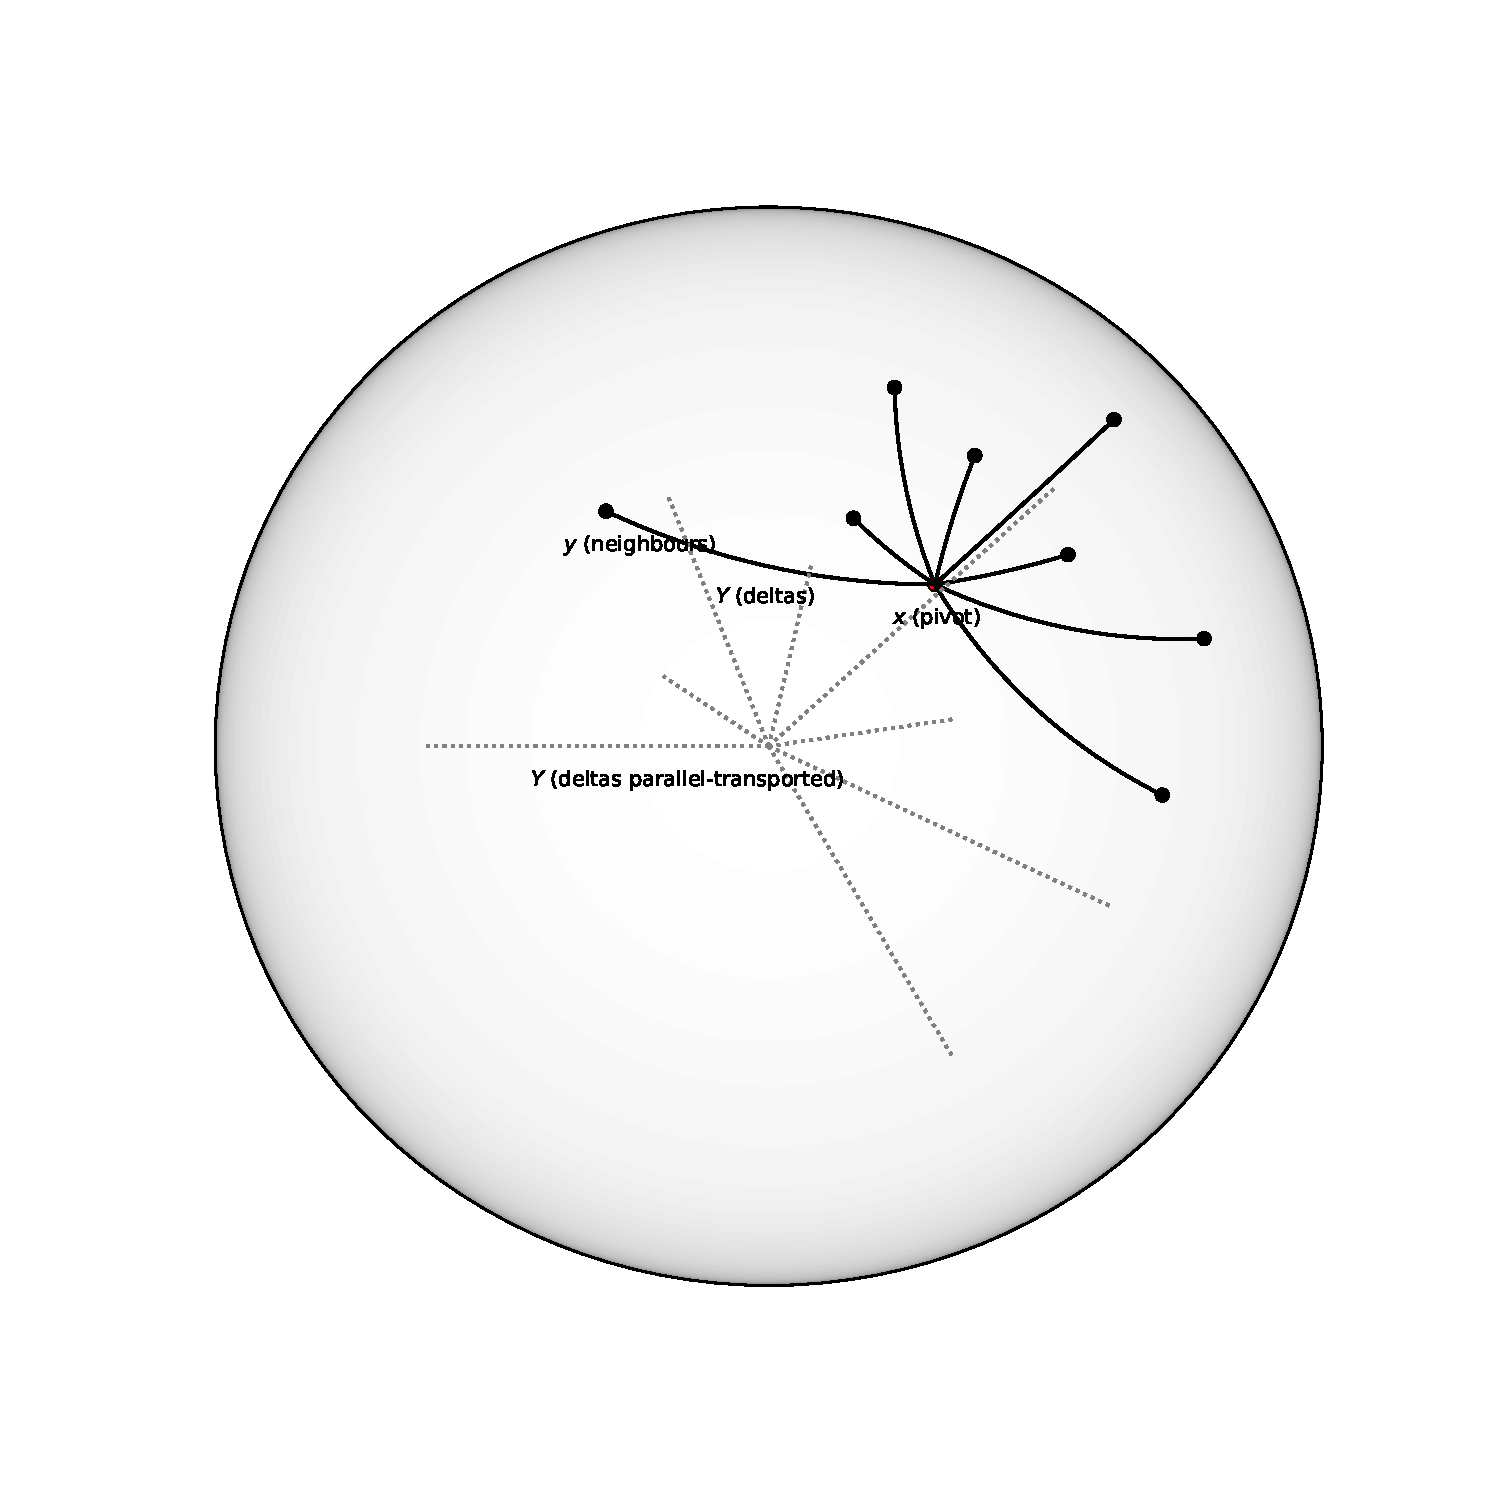
\includegraphics[width=.5\textwidth]{art/neighbours.pdf}
\caption{Relative directions to neighbour embeddings. To an embedding \( y \)
there corresponds a tangent vector \( Y = \log_x y \), visualized here as a
geodesic line segment in Poincar\'e ball.}
\end{figure}

\subsection{Hyperbolic EdgeConv} \label{sec:hedgeconv}

\citet{edgeconv} propose a convolutional layer that operates directly on
pointclouds (producing a ``cloud of embeddings'' after each step, similar to
how we produce a regular \( 2 \)D \emph{array} of embeddings in the section
above). This layer dynamically constructs a \( k \)-nearest neighbours graph
from the input pointcloud, and then transforms each point by aggregating it
with adjacent nodes. Specifically, for each neighbour of a node under
consideration, a message is constructed using an MLP that ``eats'' a point and its
location relative to the node. A pooling is then used to aggregate the messages
and produce the output point.

Replacing the subtraction with logarithmic map in message formation, and using
manifold distances when constructing \( k \)-NN graph, we can generalize the
operation to hyperbolic embeddings. A number of concerns remains: the original
model uses Batch Normalization and rectifying non-linearities. Search for
meaningful non-linearities for hyperbolic neural networks remains an open
problem. Batch Normalization is straightforwardly generalized, but only
partially: mean and variance make perfect sense in general metric space
setting, but \emph{co}variances inherently rely on the product-structure of
vector space-valued random variables.

We note that our convolutions for arrays of hyperbolic points from the previous
section are in fact an instance of such EdgeConv, if an image is treated as a
regular grid-like graph. In particular, in our implementation of EdgeConv we
allow image inputs by deleting \textrm{KNNEdges} layer that dynamically
constructs the \( k \)-NN graph from the input.

\begin{figure}[H]\center
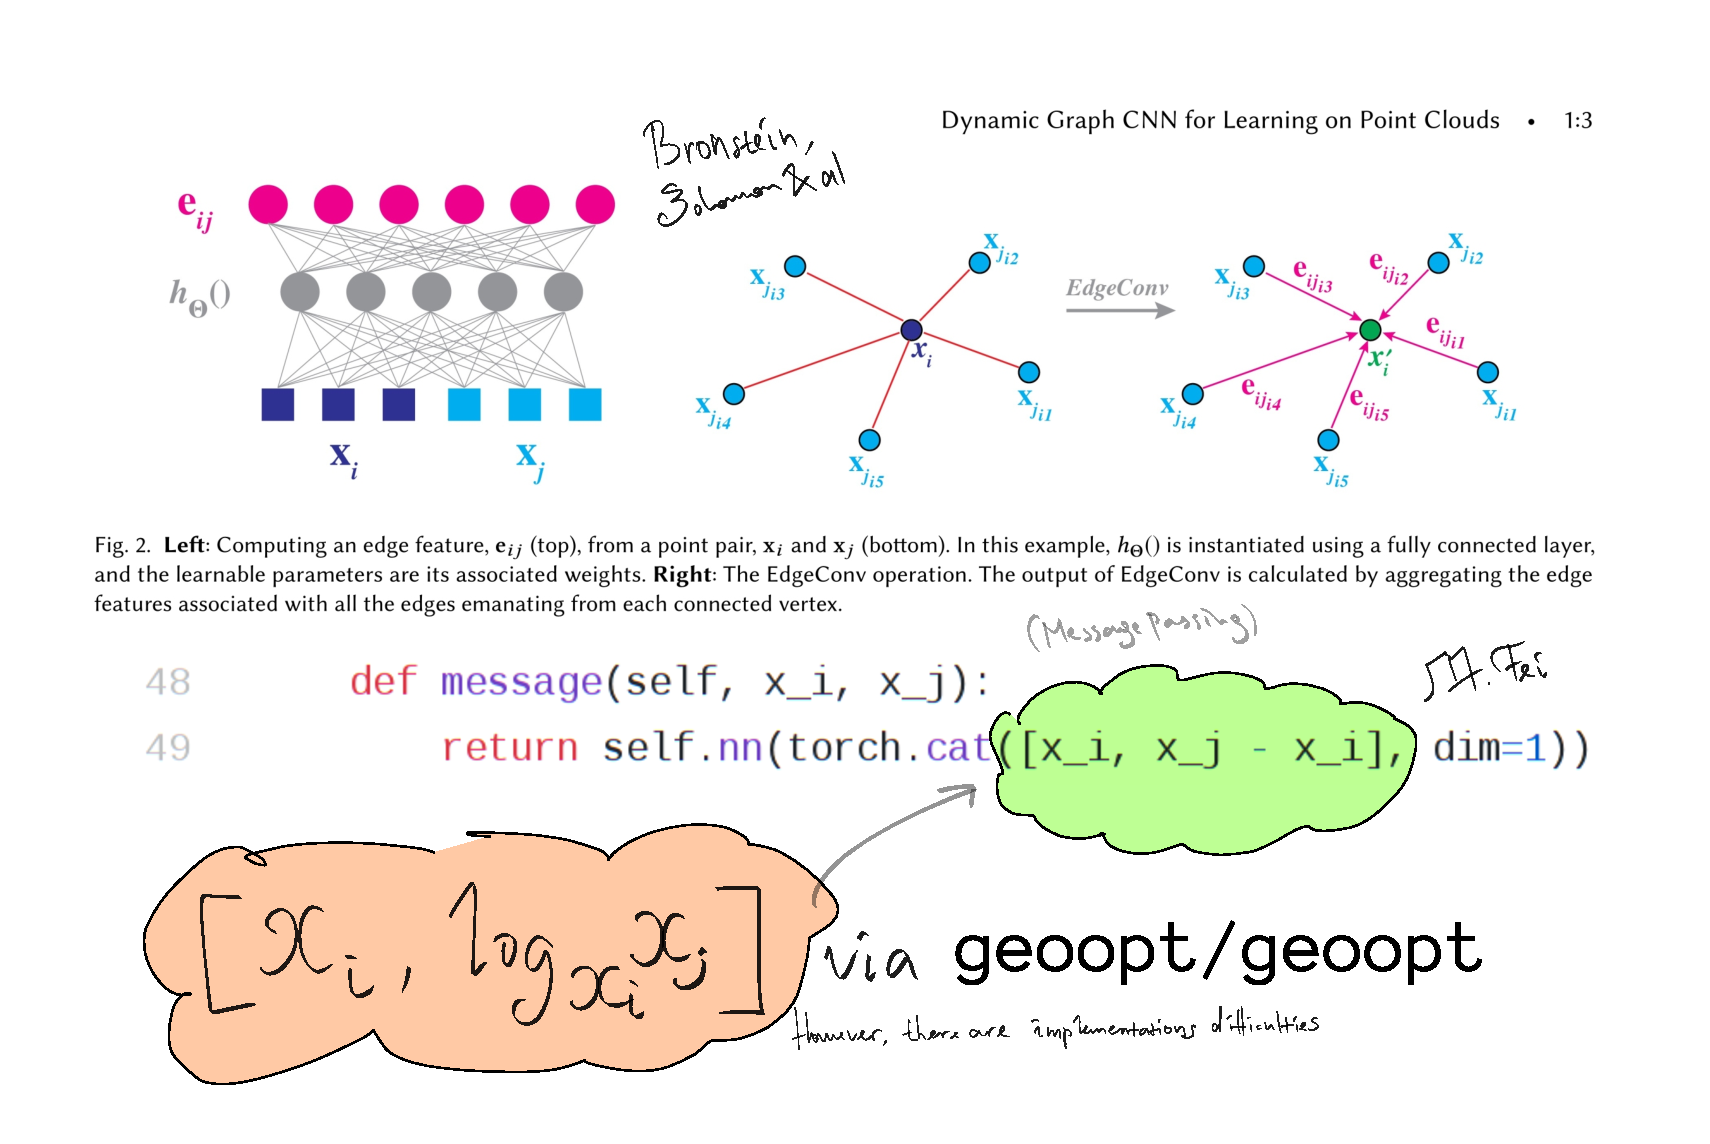
\includegraphics[width=.75\textwidth]{art/hyperbolic-edgeconv.pdf}
\caption{
    Visualization of EdgeConv from~\citet{edgeconv} and the change
        required to EdgeConv implementation of~\citet{pytorchGeometric}
}
\end{figure}

\section{Results} \label{sec:results}

Just as model in Appendix~\autoref{appendix:hconv}, our model proved to heavily
suffer from overfitting and fail to learn under reasonable regularization.  Our
naive hyperbolic edge convolution slightly under-performs compared to
baselines, but using much less parameters. However, that comes at cost of
longer iterations and so far we haven't succeeded at beating the baselines.

\section{Discussion} \label{sec:discussion}

There's a number of conceptial inconsistencies with considered models.  First
of all, in both cases the ``convolution'' happens along the spatial dimensions
(over window pixels in an image, and over graph edges in EdgeConv). The image
case is especially good at illuminating the inconsistency: our input is a
signal on Euclidean plane, and we're trying to construct an operation invariant
with respect to... what group exactly? While this is not what we did, think
what sense does M\"obius transformation of a photograph make? It's a type
mismatch.
\citet{s2cnn} carefully reformulate a problem at hand so that the input to the
model is a signal on a sphere, and apply a classic convolution equivariant with
respect to the group of rotations. Similarly, for our ``convolutions of
hyperbolic arrays'' or ``hyperbolic edge convolutions'', we shall first find an
interpretation of our input as a signal on certain space and then describe an
operation invariant (or equivariant) with respect to appropriate
transformations. Such operation should interpretable as aggregation in EdgeConv,
and also follow the inutition of the ``continuous trees'' metaphor as
in~\autoref{appendix:hconv}. In our current models we involuntarily interpret
hyperbolic points within the sliding window as a trivial hyperbolic signal (sum
of delta measures). By taking the logarithmic map from one of the points in the
window, we make our ``convolution'' invariant with respect to translations of
hyperbolic space. However we might in fact want equivariance with respect to
all unit ball-preserving M\"obius transformations (isometries of Poincar\'e disk)
and we could employ the technique similar to~\cite{s2cnn} and integrate
over the entire group of isometries. We cannot hope to implement that efficiently
without the tricks of Harmonic analysis. \citet{stollharmonic} works out the
Harmonic analysis on real Hyperbolic space, including the spherical harmonics
basis. We should also note that our singular (combination of delta measures)
signal might turn out not to be the most convenient to work with in terms of
complexity of computations, nor the most representative one. In other words, we
must reconsider the way we construct and represent a signal on a Hyperbolic
space. Finally, the problem of coming up with meaningful nonlinearities
for general manifolds and particularly Hyperbolic spaces remains open.
